\documentclass[document.tex]{subfiles}
\begin{document}
\section*{Exercise 3:}

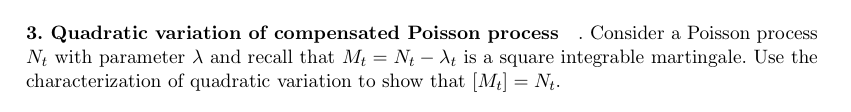
\includegraphics[width=\textwidth]{ex3.png}


We start with:
\begin{equation}
[M_t] = [N_t - \lambda t] = [N_t] - 2[N_t, \lambda t] + [\lambda t] = [N_t]
\end{equation}

The increments of $\lambda t$ go asymptotically to 0 as the size of the increments gets smaller. Therefore their covariation with $N_t$ goes to 0 as well.

We divide t into sub-intervals: $0 = t_0 < t_1 < t_2 < ... < t_n = t$ \\

We know that for sufficiently small increments $\Delta N$ is either 1 when there is a jump and 0 when there is no jump and therefore:

\begin{equation}
[N_t] = lim_{n \to \infty} \sum_{i = 1}^n (N_{t_i} - N_{t_{i - 1}})^2 = N_t
\end{equation}



\end{document}
